% Slides for lab retreat
% Author: Nishanth Koganti
% Date: 2015/7/29

\documentclass[10pt]{beamer}

\usetheme{CambridgeUS}
\usecolortheme{seahorse}
\usefonttheme{serif}

\usepackage{bm}
\usepackage{tikz}
\usepackage{color}
\usepackage{xcolor}
\usepackage{caption}
\usepackage{amssymb}
\usepackage{amsmath}
\usepackage{fancybox}
\usepackage{amsfonts}
\usepackage{listings}
\usepackage{graphicx}
\usepackage{subcaption}
\graphicspath{{./Images/}}
\usepackage[absolute,overlay]{textpos}
\usetikzlibrary{arrows,shapes,backgrounds,shapes.misc,fit,positioning}

\setbeamercovered{invisible}
%\setbeamercovered{transparent}

\newenvironment{reference}[2]{%
  \begin{textblock*}{\textwidth}(#1,#2)
    \footnotesize\it\bgroup\color{red!50!black}}{\egroup\end{textblock*}}

\everymath{\displaystyle}

\newcommand{\bx}{\mathbf{x}}
\newcommand{\by}{\mathbf{y}}
\newcommand{\ba}{\mathbf{a}}
\newcommand{\bb}{\mathbf{b}}
\newcommand{\bw}{\mathbf{w}}
\newcommand{\boldf}{\mathbf{f}}
\newcommand{\bA}{\mathbf{A}}
\newcommand{\bB}{\mathbf{B}}
\newcommand{\bC}{\mathbf{C}}
\newcommand{\gp}{\mathcal{GP}}
\newcommand{\gaussN}{\mathcal{N}}
\newcommand{\argmax}{\text{argmax}}
\newcommand{\bmu}{\boldsymbol{\mu}}
\newcommand{\bSig}{\boldsymbol{\Sigma}}

\title{Learning with Gaussian Processes using GPy}
\author{Nishanth Koganti}
\date{\today}

\begin{document}

  \begin{frame}[noframenumbering]
    \titlepage
  \end{frame}

  \begin{frame}
    \frametitle{Supervised Learning: Ubiquitous questions}

    \begin{itemize}
      \item Model fitting
      \begin{itemize}
        \item How to fit parameters?
        \item How to handle overfitting?
      \end{itemize}

      \item Model selection
      \begin{itemize}
        \item Which model best represents data?
        \item How sure can I be?
      \end{itemize}

      \item Interpretation
      \begin{itemize}
        \item What is the accuracy of predictions?
        \item Can I trust predictions under model uncertainity?
      \end{itemize}
    \end{itemize}

    \begin{center}
      \textbf{Gaussian Processes provides framework to address these issues.}
    \end{center}
  \end{frame}

  \begin{frame}
    \frametitle{Gaussian Processes: Extremely Short Overview}

    \begin{columns}
      \begin{column}{0.33\textwidth}
        Generate functions
        \begin{figure}
          \centering
          \includegraphics[width=\textwidth]{func1.png}
        \end{figure}
      \end{column}
      \pause
      \begin{column}{0.33\textwidth}
        Observe Data
        \begin{figure}
          \centering
          \includegraphics[width=\textwidth]{func2.png}
        \end{figure}
      \end{column}
      \pause
      \begin{column}{0.33\textwidth}
        Remove invalid functions
        \begin{figure}
          \centering
          \includegraphics[width=\textwidth]{func3.png}
        \end{figure}
      \end{column}
    \end{columns}
  \end{frame}

  \begin{frame}[noframenumbering]
    \frametitle{Outline}
    \tableofcontents
  \end{frame}

  \section{Gaussian Processes}
  \begin{frame}
    \frametitle{Gaussian Distribution}

    \begin{figure}
      \centering
      \includegraphics[width=0.9\textwidth]{gaussDist1.png}
    \end{figure}

    \begin{equation*}
      \begin{array}{c}
        p(\bx|\bmu,\bSig) = \gaussN(\bmu,\bSig) = (2\pi)^{-D/2} |\bSig|^{-1/2} \exp \left( - \frac{1}{2} (\bx - \bmu)^T \bSig^{-1} (\bx - \bmu) \right) \\
        \bmu \text{: mean vector, } \bSig \text{: covariance matrix}
      \end{array}
    \end{equation*}
  \end{frame}

  \begin{frame}
    \frametitle{Conditional and Marginal of a Gaussian}

    \begin{figure}
      \centering
      \includegraphics[width=\textwidth]{gaussDist2.png}
    \end{figure}

    \begin{center}
      \textcolor{blue}{Conditional} and \textcolor{red}{Marginal} of a joint Gaussian is also Gaussian.
    \end{center}

  \end{frame}

  \begin{frame}
    \frametitle{What is a Gaussian Process?}
    Generalization of a multivariate Gaussian to \textcolor{red}{infinitely many variables}.

    \begin{block}{}
      \textbf{Definition}: \emph{Gaussian Process is a collection of random variables, any finite collection of which are Gaussian Distributed.}
    \end{block}

    Gaussian \textcolor{blue}{distribution}: mean \textcolor{red}{vector}, $\bmu$, and covariance \textcolor{red}{matrix} $\bSig$:
    \begin{equation*}
      \mathbf{f} = (f_1,\dots,f_n)^T \sim \gaussN(\bmu,\bSig),~~\text{indices } i = 1,\dots,n
    \end{equation*}

    Gaussian \textcolor{blue}{process}: mean \textcolor{red}{function}, $m(x)$, and covariance \textcolor{red}{function} $k(x,x')$:
    \begin{equation*}
      f(x) \sim \gp(m(x),k(x,x')),~~\text{indices: } x
    \end{equation*}
  \end{frame}

  \begin{frame}
    \frametitle{Marginalization Property}
    How can we represent infinite mean vector and infinite covariance matrix? \\~

    ...luckily saved by \emph{marginalization property}:

    \begin{equation*}
      p(\bx) = \int p(\bx,\by)d \by
    \end{equation*}

    For Gaussians:

    \begin{equation*}
      \begin{array}{c}
        p(\bx, \by) = \gaussN \left(\begin{bmatrix} \ba \\ \bb \end{bmatrix}, \begin{bmatrix} \bA & \bB \\ \bB^T & \bC \end{bmatrix} \right) \\~\\
        p(\bx) = \gaussN(\ba,\bA)
      \end{array}
    \end{equation*}
  \end{frame}

  \begin{frame}
    \frametitle{Random sampling from Gaussian Process}
    Considering one dimensional Gaussian process:

    \begin{equation*}
      p(f(x)) \sim \gp \left( m(x) = 0, k(x,x') = \exp \left( - \frac{1}{2} (x - x')^2 \right) \right)
    \end{equation*}

    Sampling is done by focusing on subset $\boldf = (f(x_1), f(x_2),\dots,f(x_n))^T$:

    \begin{equation*}
      \boldf \sim \gaussN(0,\bSig) \text{, where } \bSig_{ij} = k(x_i,x_j)
    \end{equation*}

    Coordinates of $\boldf$ are plot as a function of corresponding $x$
  \end{frame}

  \begin{frame}
    \frametitle{Gaussian Distribution Sample}

    \begin{figure}
      \centering
      \includegraphics[width=\textwidth]{samplePath.png}
    \end{figure}
  \end{frame}

  \begin{frame}[noframenumbering]
    \frametitle{Gaussian Distribution Sample: $f1$ vs $f2$}

    \begin{figure}
      \centering
      \includegraphics[width=\textwidth]{covariance1.png}
    \end{figure}

    \begin{itemize}
      \item \textcolor{blue}{Joint distribution, $p(f_1,f_2)$}
      \item \textcolor{green}{Observation to $f_1 = -0.313$}
      \item \textcolor{red}{Conditional density, $p(f_2|f_1 = -0.313)$}
    \end{itemize}
  \end{frame}

  \begin{frame}[noframenumbering]
    \frametitle{Gaussian Distribution Sample: $f1$ vs $f5$}

    \begin{figure}
      \centering
      \includegraphics[width=\textwidth]{covariance2.png}
    \end{figure}

    \begin{itemize}
      \item \textcolor{blue}{Joint distribution, $p(f_1,f_5)$}
      \item \textcolor{green}{Observation to $f_1 = -0.313$}
      \item \textcolor{red}{Conditional density, $p(f_5|f_1 = -0.313)$}
    \end{itemize}
  \end{frame}

  \begin{frame}
    \frametitle{Squared Exponential Covariance Function}

    \begin{equation*}
      k(\mathbf{x},\mathbf{x}') = \alpha \text{exp} \left( - \frac{\|\mathbf{x} - \mathbf{x}'\|^2}{2l^2} \right)
    \end{equation*}

    where $\alpha$ is the variance and $\l$ is the length scale of the covariance function
    \begin{columns}
      \begin{column}{0.35\textwidth}
        \begin{figure}
          \centering
          \includegraphics[width=\textwidth]{kernelMatrix.png}
        \end{figure}
      \end{column}

      \begin{column}{0.45\textwidth}
        \begin{figure}
          \centering
          \includegraphics[width=\textwidth]{samplePaths.png}
        \end{figure}
      \end{column}
    \end{columns}
  \end{frame}

  \section{Inference using Gaussian Processes}

  \begin{frame}
    \frametitle{Parametric Model and Maximum Likelihood}
    Parametric Model:
      \begin{itemize}
        \item data: $\bx, \by$
        \item model: $\by = f_w(\bx) + \epsilon$
      \end{itemize}

    Gaussian Likelihood:
      \begin{equation*}
        \textcolor{red}{p(\by|\bx, \bw, M)} \propto \prod_i \exp \left( - \frac{ (y_i - f_{\bw}(x_i))^2}{2 \sigma_{noise}^2} \right)
      \end{equation*}

    Maximizing Likelihood:
      \begin{equation*}
        \bw_{ML} = \argmax_{\bw} \textcolor{red}{p(\by|\bx,\bw,M)}
      \end{equation*}

    Making predictions:
      \begin{equation*}
        p(y^*|x^*,\bw_{ML},M)
      \end{equation*}
  \end{frame}

  \begin{frame}
    \frametitle{Parametric Model and Bayesian Inference}
    Parametric Model:
      \begin{itemize}
        \item data: $\bx, \by$
        \item model: $\by = f_w(\bx) + \epsilon$
      \end{itemize}

    Gaussian Likelihood:
      \begin{equation*}
        \textcolor{red}{p(\by|\bx, \bw, M)} \propto \prod_i \exp \left( - \frac{ (y_i - f_{\bw}(x_i))^2}{2 \sigma_{noise}^2} \right)
      \end{equation*}

    Prior over parameters:
      \begin{equation*}
        \textcolor{blue}{p(\bw|M)}
      \end{equation*}

    Posterior parameter distribution:
      \begin{equation*}
        \textcolor{green}{p(\bw|\bx,\by,M)} = \frac{\textcolor{blue}{p(\bw|M)} \textcolor{red}{p(\by|\bx, \bw, M)}}{p(\by|\bx,M)}
      \end{equation*}
  \end{frame}

  \begin{frame}
    \frametitle{Parametric Model and Bayesian Inference}

    Making predictions:
      \begin{equation*}
        p(y^*|x^*,\bx,\by,M) = \int p(y^*|\bw,x^*,M) \textcolor{green}{p(\bw|\bx,\by,M)} d\bw
      \end{equation*}

    Marginal Likelihood:
      \begin{equation*}
        p(\by|\bx,M) = \int \textcolor{blue}{p(\bw|M)} \textcolor{red}{p(\by|\bx, \bw, M)} d\bw
      \end{equation*}

    Model probability:
      \begin{equation*}
        p(M|\bx,\by) = \frac{p(M)p(\by|\bx,M)}{p(\by|\bx)}
      \end{equation*}

    \begin{center}
      \textbf{Problem: integrals are intractable for most interesting models!}
    \end{center}
  \end{frame}

  \begin{frame}
    \frametitle{Non-parametric Gaussian Process Models}
    Parameters are replaced by ``function'' itself!

    Gaussian Likelihood:
      \begin{equation*}
        \textcolor{red}{\by|\bx,f(x),M} \sim \gaussN(\boldf, \sigma^2_{noise}I)
      \end{equation*}

    Gaussian Process Prior:
      \begin{equation*}
        \textcolor{blue}{f(x)|M} \sim \gp(m(x) = 0, k(x,x'))
      \end{equation*}

    Leading to Gaussian Process Posterior:
      \begin{equation*}
        \begin{array}{c}
          \textcolor{green}{f(x)|\bx,\by,M} \sim \gp ( m_{\text{post}}(x) = k(x,\bx)[K(\bx,\bx) + \sigma^2_{noise}I]^{-1} \by, \\[0.2cm]
          \; k_{\text{post}}(x,x') =  k(x,x') - k(x,\bx)[K(\bx,\bx) + \sigma^2_{noise}I]^{-1} k(\bx,x') )
        \end{array}
      \end{equation*}
    \end{frame}

  \begin{frame}
    \frametitle{Prior and Posterior for $\gp$ Learning}

    \begin{figure}
      \centering
      \includegraphics[width=\textwidth]{gpRegression.png}
    \end{figure}

    Gaussian Process Predictive Distribution:
      \begin{equation*}
        \begin{array}{c}
          p(y^*|x^*,\bx,\by) \sim \gaussN ( k(x^*,\bx)[K + \sigma^2_{noise}]^{-1}\by, \\[0.2cm]
          \; k(x*,x*) - k(x^*,\bx)[K + \sigma^2_{noise}I]^{-1} k(\bx,x^*) )
        \end{array}
      \end{equation*}
  \end{frame}

  \section{Covariance Functions}

  \begin{frame}
    \frametitle{Matern Covariance Function}

    \begin{equation*}
      k(x,x') = \frac{1}{\Gamma(\nu) 2^{\nu - 1}} \left[ \frac{\sqrt{2 \nu}}{l} |x - x'| \right]^{\nu} K_{\nu} \left( \frac{\sqrt{2 \nu}{l}} |x - x'| \right)
    \end{equation*}
    where $K_{\nu}$ is a Bessel function of order $\nu$, and $l$ is the length scale.\\~

    Samples of Matern forms are $\lfloor \nu - 1 \rfloor$ times differentiable.

    \begin{figure}
      \centering
      \includegraphics[width=0.9\textwidth]{maternCovFunc.png}
    \end{figure}

  \end{frame}

  \begin{frame}
    \frametitle{Periodic Covariance Function}
    Periodic covariance functions can be obtained by mapping $x$ to $u = (\sin(x), \cos(x))^T$ and combine with SE covariance function:

    \begin{equation*}
      k_{periodic} (x,x') = \exp \left( - \frac{2 \sin^2(\pi (x - x'))}{l^2} \right)
    \end{equation*}

    \begin{figure}
      \centering
      \includegraphics[width=0.8\textwidth]{periodicCovFunc.png}
      \caption*{3 random samples with: left $l > 1$ and right $l < 1$}
    \end{figure}
  \end{frame}

  \begin{frame}
    \frametitle{Prediction Problem}

    \begin{figure}
      \centering
      \includegraphics[width=0.8\textwidth]{prediction1.png}
    \end{figure}
  \end{frame}

  \begin{frame}
    \frametitle{Covariance Functions}

    \begin{itemize}
      \item long term smooth trend (\textcolor{blue}{squared exponential})
        \begin{equation*}
          k_1(x,x') = \theta_1^2 \exp \left( \frac{(x - x')^2}{\theta_2^2} \right)
        \end{equation*}
      \item seasonal trend (\textcolor{blue}{quasi-periodic smooth})
        \begin{equation*}
          k_2(x,x') = \theta_3^2 \exp \left( - \frac{2 \sin^2 (\pi (x - x'))}{\theta_5^2} \right) \times \exp \left( \frac{(x - x')^2}{2 \theta_4^2} \right)
        \end{equation*}
      \item short and medium term anomaly (\textcolor{blue}{rational quadratic})
        \begin{equation*}
          k_3(x,x') = \theta_6^2 \left( 1 + \frac{(x - x')^2}{2 \theta_8 \theta_7^2} \right)^{- \theta_8}
        \end{equation*}
    \end{itemize}

    \begin{equation*}
      k(x,x') = k_1(x,x') + k_2(x,x') + k_3(x,x') + \text{noise kernel}
    \end{equation*}
  \end{frame}

  \begin{frame}
    \frametitle{Carbon Dioxide Predictions}

    \begin{figure}
      \centering
      \includegraphics[width=\textwidth]{prediction2.png}
    \end{figure}
  \end{frame}

  \begin{frame}
    \frametitle{Long and Medium-term Predictions}

    \begin{figure}
      \centering
      \includegraphics[width=0.8\textwidth]{prediction3.png}
    \end{figure}
  \end{frame}

  \section{Dimensionality Reduction with GP}

  \begin{frame}
  \frametitle{Motivation for Dimensionality Reduction}

  \begin{itemize}
    \item For data with underlying ``structure'', we expect:
      \begin{itemize}
        \item Fewer distortions than dimensions.
        \item Data to lie on a low-dimensional manifold.
      \end{itemize}
    \item Conclusion: Deal with high-dimensional data by looking for low-dimensional embedding.
  \end{itemize}

  \end{frame}

  \begin{frame}
  \frametitle{Non-linear Dimensionality Reduction}

  \begin{center}
    \textbf{UPSC Handwritten Digit Dataset}
  \end{center}

  \begin{columns}[t]
    \begin{column}[t]{0.3\textwidth}
      \centering
      3648 dimensional space
      \begin{figure}
        \centering
        \caption*{Digit 6 Image}
        \includegraphics[width=0.3\textwidth]{digitIm1.png}
      \end{figure}
      \begin{figure}
        \centering
        \caption*{Random Image}
        \includegraphics[width=0.3\textwidth]{digitIm2.png}
      \end{figure}
    \end{column}
    \begin{column}{0.6\textwidth}
      \centering
      Low-dimensional manifold for digit rotation
      \begin{figure}
        \centering
        \includegraphics[width=0.8\textwidth]{pca1.png}
      \end{figure}
    \end{column}
  \end{columns}

  \end{frame}

  \begin{frame}
  \frametitle{Probabilistic Generative Model}

  \begin{itemize}
    \item \textcolor{blue}{Observed} (high-dimensional) data: $\mathbf{Y} = [y_1~y_2~\cdots~y_N]^T \in \mathbb{R}^{N \times D}$
    \item \textcolor{blue}{Latent} (low-dimensional) data: $\mathbf{X} = [x_1~x_2~\cdots~x_N]^T \in \mathbb{R}^{N \times Q},~Q << D$
    \item Assume a relationship/mapping of the form:
      \begin{equation}
        \begin{array}{c}
          y_i = \mathbf{W}x_i + \epsilon_i,~\epsilon_i \sim \mathcal{N}(\mathbf{0},\sigma^2\mathbf{I})\\~\\
          y_i = f(x_i) = \epsilon_i
        \end{array}
      \end{equation}
    \item Resultant likelihood on the data:
      \begin{equation}
        p(\mathbf{Y}|\mathbf{X},\mathbf{W}) = \prod_{i = 1}^N \mathcal{N}(y_i | \mathbf{W}x_i, \sigma^2\mathbf{I})
      \end{equation}
  \end{itemize}

  \end{frame}

  \begin{frame}
  \frametitle{Probabilistic Generative Model}

  \begin{columns}
    \begin{column}[t]{0.48\textwidth}
      \centering
      \textbf{Probabilistic PCA}
      \begin{figure}
        \centering
        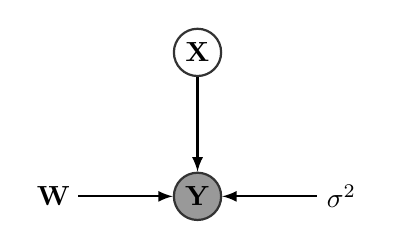
\begin{tikzpicture}
          \tikzstyle{main}=[circle, minimum size = 6mm, thick, draw =black!80, node distance = 12mm]
          \tikzstyle{main1}=[circle, minimum size = 6mm, thick, draw = white, node distance = 12mm]
          \tikzstyle{connect}=[-latex, thick]
          \node[main,fill=black!40] (y) [label=center:$\mathbf{Y}$] {};
          \node[main] (x) [above=of y,label=center:$\mathbf{X}$] {};
          \node[main1] (w) [left=of y,label=center:$\mathbf{W}$] {};
          \node[main1] (sigma) [right=of y,label=center:$\sigma^2$] {};
          \path (x) edge [connect] (y)
          (w) edge [connect] (y)
          (sigma) edge [connect] (y);
        \end{tikzpicture}
      \end{figure}
      Places prior on latent space $\mathbf{X}$ and optimises linear mapping $\mathbf{W}$
      \begin{equation}
        \begin{array}{c}
          p(\mathbf{X}) = \prod_{i=1}^N \mathcal{N}(x_i|\mathbf{0},\mathbf{I})\\~\\
          p(\mathbf{Y}|\mathbf{W},\sigma^2) = \int p(\mathbf{Y}|\mathbf{W},\mathbf{X},\sigma^2)~p(\mathbf{X})
        \end{array}
      \end{equation}
    \end{column}
    \begin{column}[t]{0.48\textwidth}
      \centering
      \textbf{Dual Probabilistic PCA}
      \begin{figure}
        \centering
        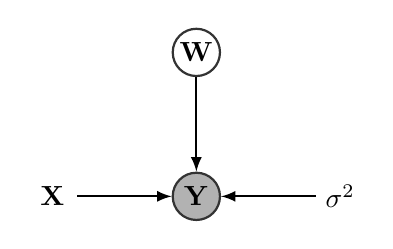
\begin{tikzpicture}
          \tikzstyle{main}=[circle, minimum size = 6mm, thick, draw = black!80, node distance = 12mm]
          \tikzstyle{main1}=[circle, minimum size = 6mm, thick, draw = white, node distance = 12mm]
          \tikzstyle{connect}=[-latex, thick]
          \node[main,fill=black!30] (y) [label=center:$\mathbf{Y}$] {};
          \node[main] (w) [above=of y,label=center:$\mathbf{W}$] {};
          \node[main1] (x) [left=of y,label=center:$\mathbf{X}$] {};
          \node[main1] (sigma) [right=of y,label=center:$\sigma^2$] {};
          \path (x) edge [connect] (y)
          (w) edge [connect] (y)
          (sigma) edge [connect] (y);
        \end{tikzpicture}
      \end{figure}
      Places prior on linear mapping $\mathbf{W}$ and optimises latent space $\mathbf{X}$
      \begin{equation*}
        \begin{array}{c}
          p(\mathbf{W}) = \prod_{i=1}^D \mathcal{N}(w_i|\mathbf{0},\mathbf{I})\\~\\
          p(\mathbf{Y}|\mathbf{X},\sigma^2) = \int p(\mathbf{Y}|\mathbf{W},\mathbf{X},\sigma^2)~p(\mathbf{W})
        \end{array}
      \end{equation*}
    \end{column}
  \end{columns}

  \end{frame}

  \begin{frame}
  \frametitle{From Dual PPCA to GP-LVM}

  \begin{exampleblock}{}
    \centering
    PPCA and Dual PPCA are equivalent eigenvalue problems with same Maximum Likelihood solution
  \end{exampleblock}

  \begin{itemize}
    \item \textcolor{blue}{GP-LVM}: Instead of placing prior $p(\mathbf{W})$ on the function parameters in Dual PPCA, we can place a prior $p(f)$ directly on the mapping function i.e. \textcolor{blue}{$\mathcal{GP}$ Prior}\\~\\
    \item A $\mathcal{GP}$ Prior allows for \textcolor{blue}{non-linear mappings} if the covariance function is non-linear. For example, the SE Covariance Function:
      \begin{equation}
        k(x,x') = \alpha~\text{exp} \left( - \frac{\gamma}{2} (x - x')^T(x - x') \right)
      \end{equation}
  \end{itemize}

  \begin{figure}
    \centering
    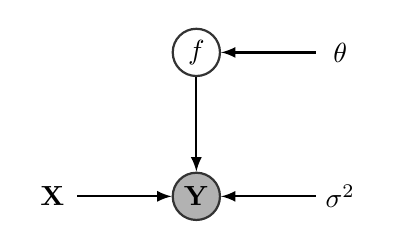
\begin{tikzpicture}
      \tikzstyle{main}=[circle, minimum size = 6mm, thick, draw = black!80, node distance = 12mm]
      \tikzstyle{main1}=[circle, minimum size = 6mm, thick, draw = white, node distance = 12mm]
      \tikzstyle{connect}=[-latex, thick]
      \node[main,fill=black!30] (y) [label=center:$\mathbf{Y}$] {};
      \node[main] (f) [above=of y,label=center:$f$] {};
      \node[main1] (theta) [right=of f,label=center:$\theta$] {};
      \node[main1] (x) [left=of y,label=center:$\mathbf{X}$] {};
      \node[main1] (sigma) [right=of y,label=center:$\sigma^2$] {};
      \path (x) edge [connect] (y)
      (f) edge [connect] (y)
      (sigma) edge [connect] (y)
      (theta) edge [connect] (f);
    \end{tikzpicture}
  \end{figure}

  \end{frame}

  \begin{frame}
  \frametitle{Difficulty with Non-linear Mapping}

  \begin{itemize}
    \item Normalization of probability distribution after passing through non-linear mapping becomes difficult:
      \begin{figure}
        \centering
        \includegraphics[width=0.5\textwidth]{nonlinear2.png}
      \end{figure}

    \item No longer possible to optimize wrt $\mathbf{X}$ as an eigen value problem
      \begin{equation}
        \mathbf{X},\theta = \text{argmax}_{\mathbf{X},\theta} p(\mathbf{Y}|\mathbf{X},\theta)
      \end{equation}

    \item Instead we need to use iterative approach and find gradients wrt $\mathbf{X},\alpha,\gamma,\sigma^2$

  \end{itemize}

  \end{frame}

  \begin{frame}
  \frametitle{Linear vs. Non-linear Dimensionality Reduction}

  \begin{figure}
    \centering
    \includegraphics[width=0.8\textwidth]{mapping.png}
  \end{figure}

  \end{frame}

  \begin{frame}
  \frametitle{Extensions of GP-LVM}

  \textbf{Back Constrained GP-LVM}: Ensures points close in the observation space ($Y$) will be close in latent space by constraining back mapping $f': Y \rightarrow X$\\~\\

  \textbf{GP-LVM with Dynamics Model}: Computes latent space assuming that the latent positions ($\mathbf{X}$) are sequential:

  \begin{equation}
    x_t = h(x_{t-1}) + \epsilon_{dyn}, \epsilon_{dyn} \sim \mathcal{N}(\mathbf{0},\sigma^2_{dyn}\mathbf{I})
  \end{equation}

  A $\mathcal{GP}$ Prior is placed on the function $h(x)$. The resultant optimization becomes:

  \begin{equation}
    \mathbf{X},\theta,\theta_{dyn} = \text{argmax}_{\mathbf{X},\theta,\theta_{dyn}}~p(\mathbf{Y}|\mathbf{X},\theta)~p(\mathbf{X}|\theta_{dyn})
  \end{equation}

  \end{frame}

  \begin{frame}
    \frametitle{Conclusions}

    \textbf{Complex non-linear inference problems can be solved by manipulating plain old Gaussian Distributions}

    \begin{itemize}
      \item Bayesian inference is tractable for GP Regression
      \item Predictions are probabilistic
    \end{itemize}

    \textbf{Scope for research:}

    \begin{itemize}
      \item Interesting covariance functions
      \item Application to high-dimensional data (Deep Learning)
    \end{itemize}

  \end{frame}

  \begin{frame}[noframenumbering]
    \frametitle{Optimizing Marginal Likelihood}
    \begin{equation*}
      \log p(\by|\bx,M) = - \textcolor{blue}{\frac{1}{2} \by^T K^{-1} \by} - \textcolor{red}{\frac{1}{2} \log|K|} - \frac{n}{2} \log (2\pi)
    \end{equation*}

    is a combination of \textcolor{blue}{data fit} and \textcolor{red}{complexity penalty} terms. Occam's razor is automatic!\\~\\

    \textcolor{blue}{Learning} in Gaussian process models involves finding:
      \begin{itemize}
        \item Form of covariance matrix
        \item Unknown hyperparameter values $\theta$
      \end{itemize}

    ~\\ This can be done by optimizing the marginal likielihood:

    \begin{equation*}
      \frac{\partial \log p(\by|\bx,\theta,M)}{\partial \theta_j} = \frac{1}{2} \by^T K^{-1} \frac{\partial K}{\partial \theta_j} K^{-1} \by - \frac{1}{2} \text{trace} \left( K^{-1} \frac{\partial K}{\partial \theta_j} \right)
    \end{equation*}
  \end{frame}

  \begin{frame}[noframenumbering]
    \frametitle{Example: Length Parameter Learning}

    Covariance function: $k(x,x') = \nu^2 \exp \left( - \frac{(x - x')^2}{2l^2} \right) + \sigma_{noise}^2 \delta_{xx'}$

    \begin{figure}
      \centering
      \includegraphics[width=0.8\textwidth]{gpLearning.png}
    \end{figure}

    Posterior mean function is plotted for 3 different length scales, green curve maximizes marginal likelihood. \textcolor{blue}{Although exact fit for data can be found, marginal likelihood does not favour this!}
  \end{frame}

  \begin{frame}[noframenumbering]
    \frametitle{Why does Bayesian Inference work?: Occam's Razor}

    \begin{figure}
      \centering
      \includegraphics[width=0.9\textwidth]{occamsRazor.png}
    \end{figure}
  \end{frame}
\end{document}
